\documentclass{article}
\usepackage[utf8]{inputenc}
\usepackage{graphicx}
%\usepackage{subfig}
\usepackage{caption, subcaption}
\usepackage[colorlinks]{hyperref}
\usepackage{textcomp}

%\catcode`\_=\active
%\def_#1_{\emph{#1}}
%\catcode``=\active
%\def`#1`{{\tt#1}}

\title{Machine Learning for Computer Vision\\ Handwritten Math Recognition}
\author{Harold Mouchère}
\date{\today}


\begin{document}
\newcommand{\xmlelt}[1]{$<$#1$>$}

\maketitle

\section{Context}

The aim of this project is to show that deeplearning tools (MLP, CNN, ...) are often embedded in a more complex problem.
Here the problem is "Recognition of On-line Handwritten Mathematical Expression" (ROHME), which is one of the task of the CROHME competitions. 

In this document, the main aspect of the project are presented, but you have to define your own solution.

\section{Inputs and Outputs}
The inputs and outputs for this exercice will be those required for the CROHME competition. By this way, you will be able to use the (python) tools provided in the competition kit.

\subsection{Inputs: Inkml}

Ink traces with ground-truth information providing the segmentation of strokes into symbols and the symbol layout are provided in the InkML format. 
Each expression is stored in one InkML file. 
This XML language is defined by the W3C (\url{http://www.w3.org/TR/InkML/}) and can easily be extended. 
A CROHME InkML file contains: 
\begin{enumerate}
\item  Ink traces: X and Y coordinates of each point sampled nearly equally in time, grouped into strokes with XML identifiers, 
\item  information about the sample and the writer: unique identifier of the expression (IUD), writer identifier, writer age, gender and handedness if available, and finally 
\item  ground-truth. 
\end{enumerate}
The ground-truth contains the following:
LaTeX string: often a rendering of this string was shown to the writer when the formula was written,
MathML (http://www.w3.org/Math/) representation of the expression using the Presentation encoding, representing the layout of symbols (with their XML identifiers) on baselines, and not their mathematical semantics,
Segmentation of strokes into groups with a symbol label and XML identifier; each segment (symbol) is linked to its corresponding MathML symbol by the symbol’s identifier.
This format contains all the necessary information needed for training a system. 
Ground-truth information is removed from test files.

Figure \ref{figInk}(a) displays the ink traces as written by the user. The ground truth information defining the ME "2+2" with its layout is represented in MathML in Figure\ref{figInk}(b). The \xmlelt{mrow} tag represents that the contained children are on the same baseline (row). \xmlelt{mn} and \xmlelt{mo} tags define numbers and operators. An additional section in the InkML file contains the segmentation information, which is not shown in Figure \ref{figInk}.
 Each group of strokes belonging to a symbol are assigned the same label, comprised of the symbol class, ‘\_’ and an index to distinguish multiple occurrences of a symbol (e.g. ‘2\_1’ and ‘2\_2’ in Figure \ref{figInk}(b)).
\begin{figure}
\begin{subfigure}{0.45\linewidth}

\includegraphics[width=\linewidth]{2plus2.png}
\caption{Ink}
\end{subfigure}
\begin{subfigure}{0.45\linewidth}
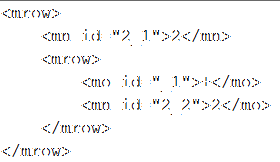
\includegraphics[width=\linewidth]{2p2mml.png}
\caption{MathML}
\end{subfigure}
\caption{ A simple handwritten expression with four strokes (a), its representation of symbol layout using MathML (b).
\label{figInk}}
\end{figure}


Inkml files can be rendered with this webbased tool inkml\_viewer available  \href{https://uncloud.univ-nantes.fr/index.php/s/OdAtErZgxKGjsNy}{here}.

\subsection{Output: LG}
LG handles for "Labelled Graph". A handwritten expression can be represented by a labeled graph, where nodes are strokes and edges represent relationships between strokes and symbols. Figure \ref{figLG} provides an example of how label graphs are defined.

\begin{figure}
\begin{subfigure}{0.45\linewidth}
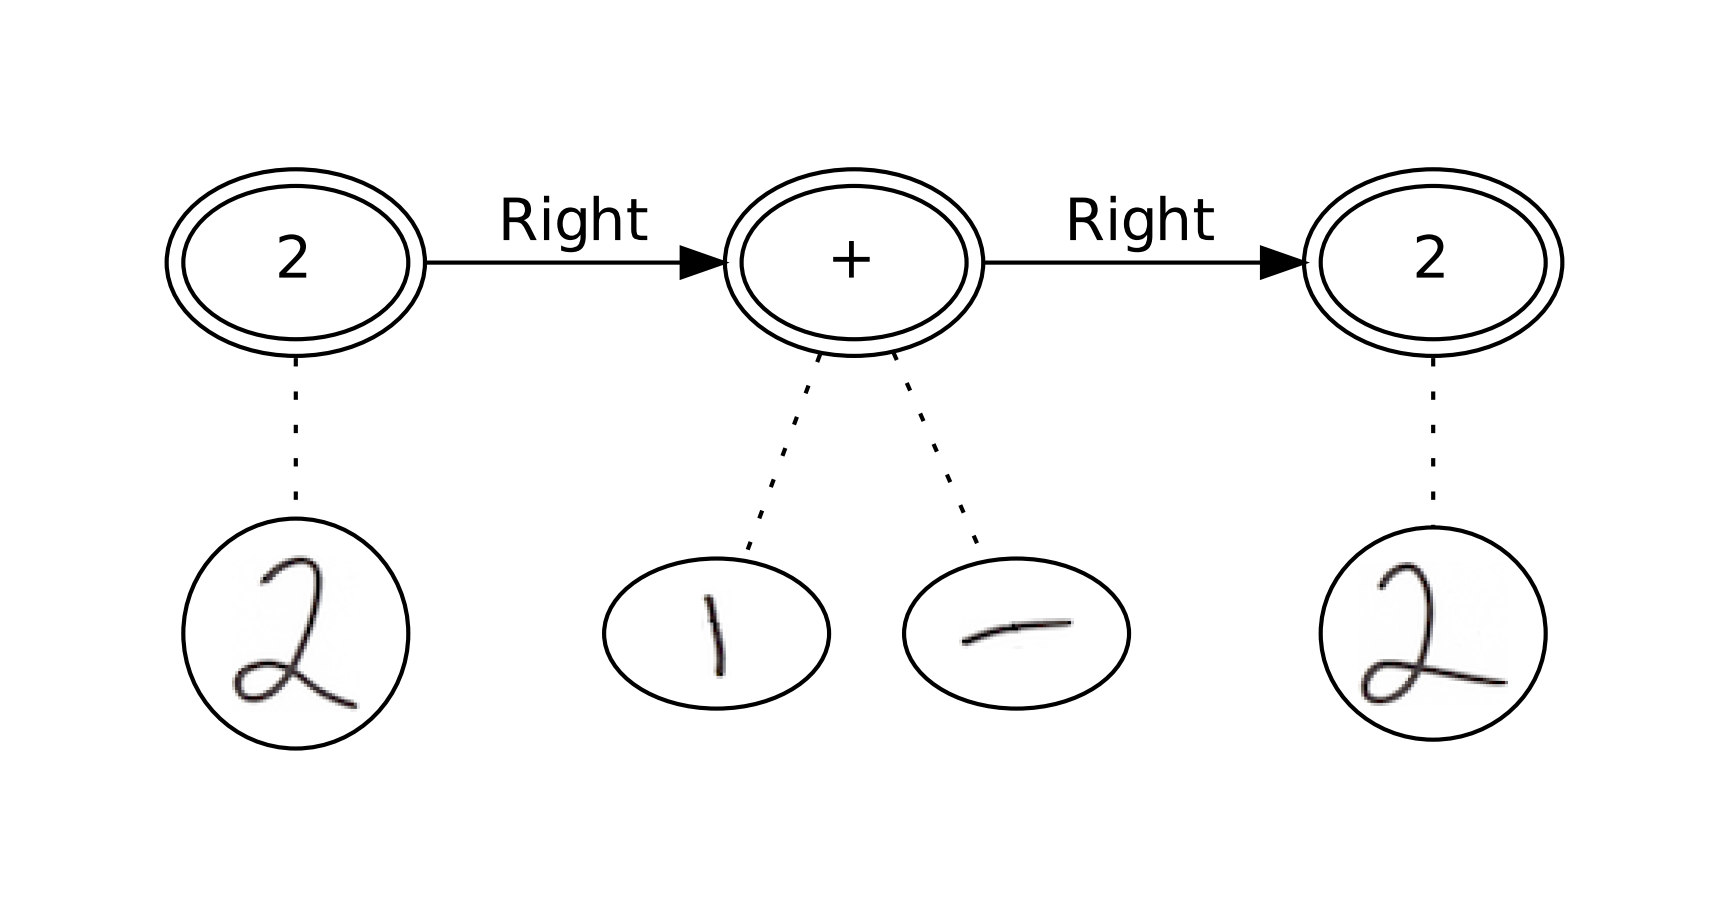
\includegraphics[width=\linewidth]{twolevel.png}
\caption{SRT}
\end{subfigure}
\begin{subfigure}{0.45\linewidth}
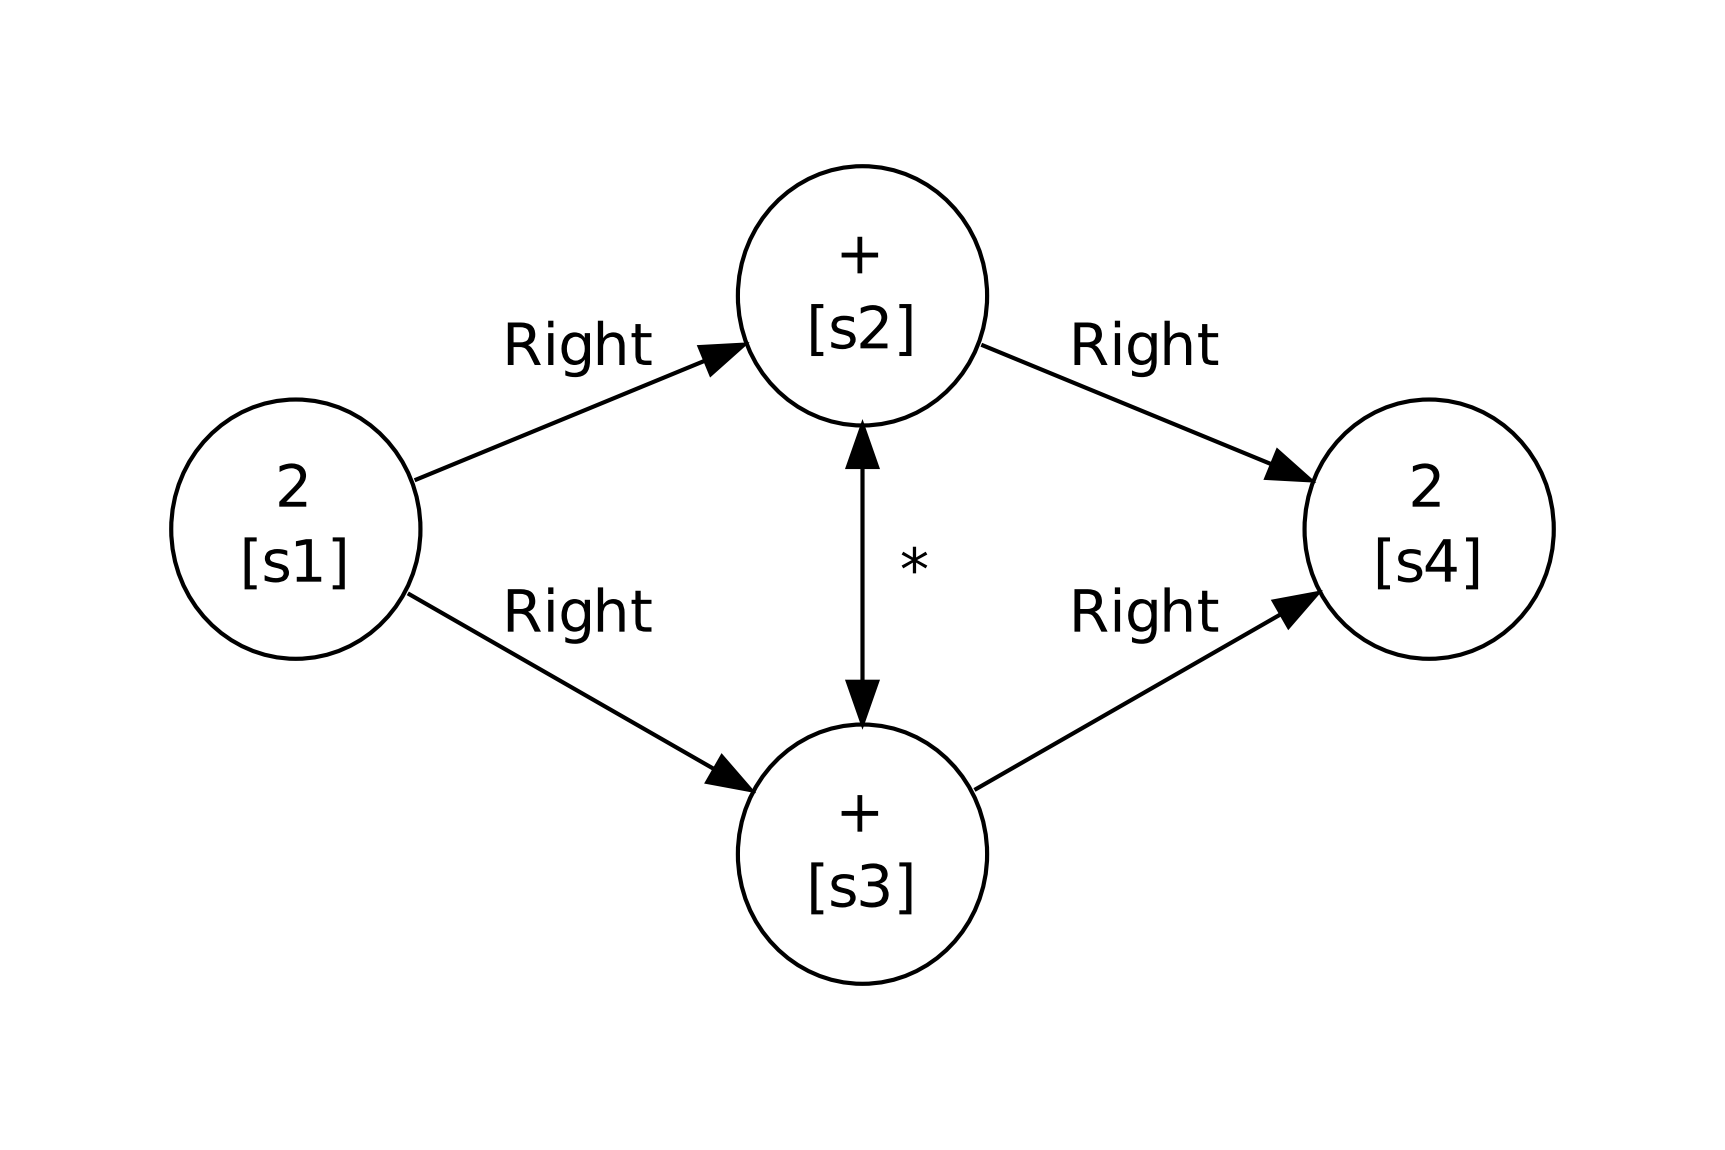
\includegraphics[width=\linewidth]{layout_lg.png}
\caption{LG}
\end{subfigure}
\caption{The symbol layout for the same handwritten expression with four strokes (a), and the stroke label graph (b).
\label{figLG}}
\end{figure}



From the MathML tree, we can create a symbol relation tree (SRT). Five relations are defined: Right, Above, Below, Sup, Sub and Inside. In Figure \ref{figLG}(a) we can see the two "Right" relationships between the three symbols (shown as nodes with double circles), defined by \xmlelt{mrow} tags in Figure \ref{figInk}(b). Each symbol is associated with its corresponding strokes (shown by dotted edges in Figure \ref{figLG}(a)). From this SRT, the layout graph of strokes can be constructed using the same spatial relation edges plus segmentation edges as in Figure \ref{figLG}(b). The segmentation edges were labeled by ‘*’ in 2013, but in this project, as in the 2014 competition, segmentation edges are labeled with the label of the corresponding symbol.
Nodes (strokes) from the same symbol are fully connected (i.e. form a clique), and share the same label. This allows several levels of segmentation in the same graph, with multiple labels on edges and nodes. This feature was used to define the matrix recognition task (the levels were: symbol, cell, row, column, and matrix).

The LG file format for label graphs was designed to be as simple as possible, human-readable, and easily used in any programming language. As shown in Figure~\ref{figLGF}, the graph is defined by a list of nodes and edges in a Coma Separated Values (CSV) text file. Nodes are defined using stroke identifiers (matching stroke identifiers in the InkML file), and a label. Edges are defined using the node identifiers they connect and a spatial relation or segmentation label. The last value of each line indicates a confidence value for the given label (symbol or relation). For the ground-truth files, these values are always 1.

\begin{figure}
\begin{subfigure}{0.5\linewidth}
\begin{verbatim}
N, s1, 2, 1.0
N, s2, +, 1.0
N, s3, +, 1.0
N, s4, 2, 1.0
E, s1,s2, Right, 1.0
E, s1,s3, Right, 1.0
E, s2,s3, +, 1.0
E, s3,s2, +, 1.0
E, s2,s4, Right, 1.0
E, s3,s4, Right, 1.0
\end{verbatim} 
\caption{Normal}
\end{subfigure}
\begin{subfigure}{0.5\linewidth}
\begin{verbatim}
O, sym1, 2, 1.0, s1
O, sym2, +, 1.0, s2, s3
O, sym3, 2, 1.0, s4
R, sym1,sym2, Right, 1.0
R, sym2,sym3, Right, 1.0
\end{verbatim}
\caption{Short}
\end{subfigure}
\caption{The two versions of the same LG file for the expression "2+2" of Figure \ref{figLG}(b).
\label{figLGF}}
\end{figure}

\subsection{Evaluation}
Evaluation is performed by comparing the respective label graphs for the ground-truth and your system output. 
Consequently, your system should output LG files. 

The provided evaluation allows to measure the recall and precision of node (stroke)'s  labels and edge (relation)'s labels. Furthermore, it also compute recall and precision metric at the symbol level considering the segmentation deduced from your LG file. Thus, remember to produce valid LG files with fully connected nodes of symbols.

The script to use is \texttt{evaluate} which can evaluate two complete directories (all files) of a partial list of files.

\section{Global recognition process}

This section describes briefly the 3 main steps of a ROHME.
\subsection{Segmentation}
This step consists in grouping the strokes to form hypotheses of symbols. 
It should be noted that in on-line expression, most of  the symbols are written with consecutive strokes, but sometimes there are "delayed strokes" which come back to complete an existing stroke. 

Thus, two main strategies are possible:
\begin{enumerate}
\item stroke order dependent: the ROHME is able to recognize only symbol written with consecutive strokes;
\item stroke order free system: the ROHME is able to deal with symbols written with multi-strokes symbols not written consecutively; you can reduce the complexity by adding constraints as allowing only one "time jump" in a symbol.
\end{enumerate}

You can use a segmentation classifier to decide if an hypothesis should be kept or not. This is not mandatory.


\subsection{Recognition}

This step is simply an isolated symbol recognition task. Each hypothesis of symbol should be recognized and associated to one of several labels.

Several classifiers can be used: HMM using the time information of the strokes, MLP using extracted features, or a CNN using a image version of the symbol. The CNN solution is the simplest. The classifier can also have a reject class (junk) to reject samples which are probably wrong segmentations. 

You can use the `CROHME-train-iso.py` script as an example of symbol classifier.

The output of this step can be save in a "short version" of LG file: one file per expression, one line per symbol hypothesis (the same hypothesis can appear several times with different labels).

\subsection{Layout Analysis}
Depending of your progress, this step can be skipped.

This step recognizes the spatial relation between 2 hypothesis of symbols among: Right, Sub, Sup, Above, Below, Inside.

This recognition is generally based on features extracted from the bounding boxes of each symbol (difference of baseline, of height, distances...) with a simple classifier (SVM or MLP). It exists also some image based solutions using an image containing both symbols in the same small image (high resolution is not needed of that).

The output of this step can be saved by just add "R" relations in a "short version" LG files.

\subsection{Final decision}

Normally this step should use a grammar or another language model to select the best complete and valid expression using the available strokes and hypothesis (symbols + relations).

In the frame of this project, your system should use a strategy to select the set of symbols and relations which minimizes the global cost of the expression (sum of all costs of used symbols and relations). You can propose a greedy algorithm or a dynamic programming solution. If you have not recognized the spatial relations, used simply Right relations between ordered symbols.

The simplest appraoch is a greedy algorithm which select the best symbol hypothesis, then remove all incompatible hypothesis (because of the used strokes) and repeat until the set of remaining strokes is empty.
\section{Data}
The CROHME dataset is available from TC11 (Technical Committee 11, Reading Systems) website on  \href{http://tc11.cvc.uab.es/datasets/ICFHR-CROHME-2016_1}{CROHME's page}
\footnote{or full expressions and isolated symbol datasets can be downloaded locally \href{https://uncloud.univ-nantes.fr/index.php/s/OdAtErZgxKGjsNy}{here}}.
You will find this content:
\begin{itemize}
\item Full expressions inkml and LG files split in Train, Validation and Test;
\item Isolated symbol samples split in train, validation and test sets. Note that each isolated sample come from an existing full expression.
\end{itemize}
\section{Tools}

Both libraries `lgeval` and `crohmelib` are available on-line on extradoc or uncloud. Remember to define the environment variable, as explain in the documentation:
\begin{verbatim}
        export CROHMELibDir=[path_to_CROHMELib]
        export LgEvalDir=[path_to_LgEval]
        export PATH=$PATH:$CROHMELibDir/bin:$LgEvalDir/bin 
\end{verbatim} 

For each tool, a short documentation is available in the sources or if you call it without any parameter.

We provide a global chain process in several steps:
\begin{itemize}
\item \texttt{ segmenter.py }: Generate from an inkml file hypotheses of symbol in a LG file
\item \texttt{segmentSelect.py} : Keep or not each segment hypotheses and generate a new LG file 
\item \texttt{symbolReco.py} : Recognize each hypothesis and save all acceptable recognition in a LG file
\item \texttt{selectBestSeg.py} : From an LG file with several hypotheses, keep only one coherent global solution (greedy sub-optimal)
\end{itemize}

To run an evaluation, you will need the tool \texttt{`evaluate`} from \texttt{`lgeval`} which will compare 2 directories containing both LG files, one with ground-truth files, the other with your output. If you want to evaluate a subpart of the dataset, you have to build the list of corresponding files with \texttt{`listExistingLG.sh`}

\end{document}
